\documentclass[12pt,twoside]{report}
\usepackage[utf8x]{inputenc}

%%%%%%%%%%%%%%%%%%%%%%%%%%%%%%%%%%%%%%%%%%%%%%%%%%%%%%%%%%%%%%%%%%%%%%%%%%%%%

% Definitions for the title page
% Edit these to provide the correct information
% e.g. \newcommand{\reportauthor}{Timothy Kimber}

\newcommand{\reporttitle}{Evaluation of Various Entangling Gates for Trapped Ion Quantum Computers}
\newcommand{\projectcode}{QOLS-Thompson-1}
\newcommand{\supervisor}{Prof. Richard Thompson}
\newcommand{\degreetype}{MSci Physics}
%\newcommand{\partner}{Zhang Rongjie}
\newcommand{\CID}{01496799}
\newcommand{\assessor}{Dr. Steve Kolthammer}

%%%%%%%%%%%%%%%%%%%%%%%%%%%%%%%%%%%%%%%%%%%%%%%%%%%%%%%%%%%%%%%%%%%%%%%%%%%%%

% load some definitions and default packages
%%%%%%%%%%%%%%%%%%%%%%%%%%%%%%%%%%%%%%%%%
% University Assignment Title Page 
% LaTeX Template
% Version 1.0 (27/12/12)
%
% This template has been downloaded from:
% http://www.LaTeXTemplates.com
%
% Original author:
% WikiBooks (http://en.wikibooks.org/wiki/LaTeX/Title_Creation)
%
% License:
% CC BY-NC-SA 3.0 (http://creativecommons.org/licenses/by-nc-sa/3.0/)
% 
%
%%%%%%%%%%%%%%%%%%%%%%%%%%%%%%%%%%%%%%%%%
%----------------------------------------------------------------------------------------
%	PACKAGES AND OTHER DOCUMENT CONFIGURATIONS
%----------------------------------------------------------------------------------------
\usepackage[a4paper,hmargin=2.5cm,vmargin=2cm,includeheadfoot]{geometry}
\usepackage{textpos}
\usepackage{cite} % for bibliography
\usepackage{tabularx,longtable,multirow,subcaption,caption,wrapfig}%hangcaption
\usepackage{fncylab} %formatting of labels
\usepackage{fancyhdr} % page layout
\usepackage{url} % URLs
\usepackage[english]{babel}
\usepackage{amsmath}
\usepackage{amsfonts}
\usepackage{graphicx}
\usepackage{dsfont}
\usepackage{epstopdf} % automatically replace .eps with .pdf in graphics
\usepackage{backref} % needed for citations
\usepackage{array}
\usepackage{latexsym}
\usepackage[pdftex,pagebackref,hypertexnames=false,colorlinks]{hyperref} % provide links in pdf

\hypersetup{pdftitle={},
  pdfsubject={}, 
  pdfauthor={},
  pdfkeywords={}, 
  pdfstartview=FitH,
  pdfpagemode={UseOutlines},% None, FullScreen, UseOutlines
  bookmarksnumbered=true, bookmarksopen=true, colorlinks,
    citecolor=black,%
    filecolor=black,%
    linkcolor=black,%
    urlcolor=black}

\usepackage[all]{hypcap}


%\usepackage{color}
%\usepackage[tight,ugly]{units}
%\usepackage{float}
%\usepackage{tcolorbox}
%\usepackage[colorinlistoftodos]{todonotes}
% \usepackage{ntheorem}
% \theoremstyle{break}
% \newtheorem{lemma}{Lemma}
% \newtheorem{theorem}{Theorem}
% \newtheorem{remark}{Remark}
% \newtheorem{definition}{Definition}
% \newtheorem{proof}{Proof}


%%% Default fonts
\renewcommand*{\rmdefault}{bch}
\renewcommand*{\ttdefault}{cmtt}



%%% Default settings (page layout)
\setlength{\parindent}{0em}  % indentation of paragraph

\setlength{\headheight}{14.5pt}
\pagestyle{fancy}
\renewcommand{\chaptermark}[1]{\markboth{\chaptername\ \thechapter.\ #1}{}} 

\fancyfoot[ER,OL]{\sffamily\textbf{\thepage}}%Page no. in the left on odd pages and on right on even pages
\fancyfoot[OC,EC]{\sffamily }
\renewcommand{\headrulewidth}{0.1pt}
\renewcommand{\footrulewidth}{0.1pt}
\captionsetup{margin=10pt,font=small,labelfont=bf}


%--- chapter heading

\def\@makechapterhead#1{%
  \vspace*{10\p@}%
  {\parindent \z@ \raggedright \sffamily
    \interlinepenalty\@M
    \Huge\bfseries \thechapter \space\space #1\par\nobreak
    \vskip 30\p@
  }}

%---chapter heading for \chapter*  
\def\@makeschapterhead#1{%
  \vspace*{10\p@}%
  {\parindent \z@ \raggedright
    \sffamily
    \interlinepenalty\@M
    \Huge \bfseries  #1\par\nobreak
    \vskip 30\p@
  }}

\allowdisplaybreaks

\newcommand{\der}[3][]{\frac{\text{d}^{#1}#2}{\text{d}#3^{#1}}}
\newcommand{\partder}[3][]{\frac{\partial^{#1}#2}{\partial#3^{#1}}}
\newcommand{\expon}[2]{#1\cdot 10^{#2}}
\newcommand{\figref}[1]{Figure \ref{#1}}
\newcommand{\eref}[1]{Equation \eqref{#1}}
\newcommand{\tabref}[1]{Table \ref{#1}}
\newcommand{\result}[3]{$#1 \pm #2\,\text{#3}$}
\newcommand{\resexp}[4]{$\expon{(#1 \pm #2)}{#4}\,\text{#3}$}
\newcommand{\absresult}[3]{$\mathbf{#1 \pm #2\,\text{#3}}$}
\newcommand{\absresexp}[4]{$\mathbf{\expon{(#1 \pm #2)}{#4}\,\text{#3}}$}

\usepackage[export]{adjustbox}
\usepackage{pdfpages}
\usepackage{pgf}
\usepackage{relsize}
\usepackage{hyperref}

\graphicspath{{Images/}}

% load some macros
%\input{notation}

\date{May 2022}

\begin{document}

% load title page
% Last modification: 2015-08-17 (Marc Deisenroth)
\begin{titlepage}

\newcommand{\HRule}{\rule{\linewidth}{0.5mm}} % Defines a new command for the horizontal lines, change thickness here


%----------------------------------------------------------------------------------------
%	LOGO SECTION
%----------------------------------------------------------------------------------------


\includegraphics[width = 6cm]{./imperial}\\[0.5cm] 

\center % Center remainder of the page

%----------------------------------------------------------------------------------------
%	HEADING SECTIONS
%----------------------------------------------------------------------------------------

\textsc{\Large Imperial College London}\\[0.5cm] 
\textsc{\large Department of Physics}\\[0.5cm] 

%----------------------------------------------------------------------------------------
%	TITLE SECTION
%----------------------------------------------------------------------------------------

\HRule \\[0.4cm]
{ \huge \bfseries \reporttitle}\\ % Title of your document
\HRule \\[1.5cm]
 
%----------------------------------------------------------------------------------------
%	AUTHOR SECTION
%----------------------------------------------------------------------------------------

\begin{minipage}{0.4\textwidth}
\begin{flushleft} \large
\emph{Author CID:}\\
\CID\\
\vspace*{1em}
\emph{Project code:}\\
\projectcode
\end{flushleft}
\end{minipage}
~
\begin{minipage}{0.4\textwidth}
\begin{flushright} \large
\emph{Supervisor:} \\
\supervisor\\ % Supervisor's Name
\vspace*{1em}
\emph{Assessor:}\\
\assessor
\end{flushright}
\end{minipage}\\[4cm]

\vspace*{2em}
\begin{center}
	\emph{Word Count:}\\
	8019
\end{center}

%----------------------------------------------------------------------------------------
%	FOOTER & DATE SECTION
%----------------------------------------------------------------------------------------
\vfill % Fill the rest of the page with whitespace
Submitted as part of 
\degreetype~degree of Imperial College London\\[0.5cm]

\makeatletter
\@date 
\makeatother


\end{titlepage}




% page numbering etc.
\pagenumbering{roman}
\clearpage{\pagestyle{empty}\cleardoublepage}
\setcounter{page}{1}
\pagestyle{fancy}

\fancyhead[RE,LO]{\sffamily {\large\textbf{Improving the Reliability of Trapped Ion Quantum Computers}}}

{%\small
	\vspace*{-2.em}
	The weird world of quantum physics may be the next breakthrough in computation. But what can quantum computers do that classical ones cannot? Exploiting their unique properties we can create more efficient algorithms for many computational challenges. The most well known example is integer factorisation for which the runtime on classical computers scales as an exponential function of the size of the number being factorised. This exponential increase however can be overcome by using Shor's algorithm, which can only be implemented on quantum computers.
	
	A classical computer's internal state can be represented as a series of bits, each of which can be $0$ or $1$. The difference in quantum computers is that it stores data in qubits, the quantum analogue of the bit. While only measured as either $0$ or $1$ the outcome of measuring a qubit is probabilistic and in between measurements we can manipulate these probabilities. This state where we are uncertain about the state we'll see when we measure the qubit is referred to as superposition. The most important thing however is that this probability can also be conditional on the state of other qubits in our computer, which is referred to as entanglement. As an example, with two qubits one can create something called a Bell state, where there is an equal probability of measuring each qubit as $0$ or $1$, but either of them is measured $0$ then the other one will be guaranteed $0$ as well. Conversely, if either of them is measured as $1$, then the other will be $1$.
	
	\begin{wrapfigure}{r}{0.4\linewidth}
		\centering
		\vspace*{-0.75em}
		\hspace*{-0.5em}
		\begin{tabular}{c}
			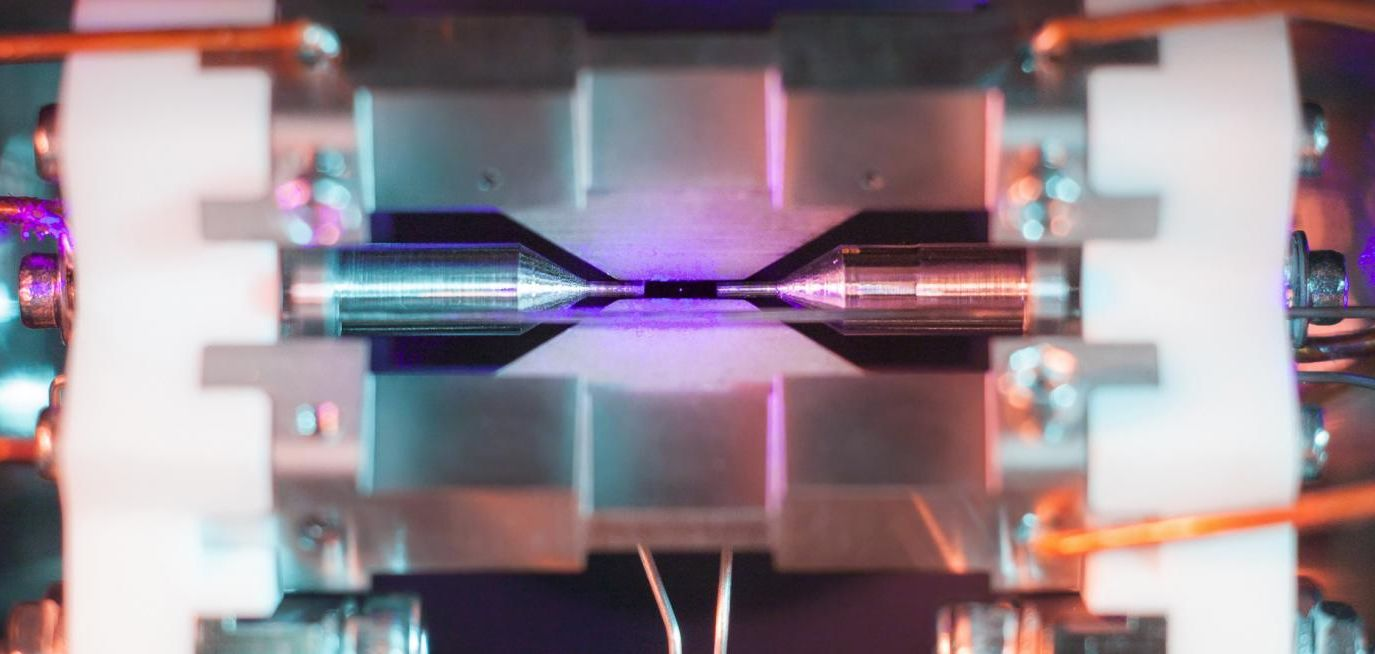
\includegraphics[width=0.95\linewidth]{TIQC.jpg}\\
			\vspace*{-.5em}\\
			\parbox{\linewidth}{\centering\footnotesize A trapped ion at the University of Oxford Ion trap quantum computing research group. Picture taken from their website\footnotemark.}
		\end{tabular}
		\vspace*{-0.75em}
	\end{wrapfigure}
	
	It is very important therefore to ensure that the qubits can be manipulated reliably. To achieve this one needs a relatively stable quantum state that can be used as the qubits and some stable way of sharing information between, manipulating and measuring these qubits to implement quantum algorithms reliably. A promising avenue toward implementation is by using trapped ions. These are charged atomic particles that are confined using magnetic and electric fields. Their internal electronic structure is ideal for use as qubits, while their back and forth motion in the trap is shared between all the ions present. As these ions are cooled to a few millionths of a Kelvin above absolute zero, this motion takes on a quantum nature, meaning that the ions' motion will only have discrete energies. This makes it a very convenient way of facilitating entanglement between them. Combination of Lasers addressing the ions can then be used to facilitate transfer between the various qubit states.
	
	In our MSci project, we simulated how different combinations of lasers, called driving schemes, can improve the reliability of a quantum computer. We did this to set expectations and give guidance to an upcoming experiment, where these schemes will be tested on a physical system. Because of this our main focus was how we can mitigate against experimental errors that inevitably arise and reduce the reliability of the qubits' state. These come from a variety of sources like the temperature and degree to which the ions can be confined. To find the best setup for the experiment we evaluated different driving schemes aimed to address the specific problems a physical system might face and have given recommendation on which ones to use. We also shown that several of these schemes could be combined giving improved performance. We hope that the increased reliability of these schemes will be demonstrated in the following years.
}
\vspace*{\fill}

\footnotetext[1]{\href{https://www.physics.ox.ac.uk/research/group/ion-trap-quantum-computing}{https://www.physics.ox.ac.uk/research/group/ion-trap-quantum-computing}}
\newpage

\fancyhead[RE,LO]{}
%%%%%%%%%%%%%%%%%%%%%%%%%%%%%%%%%%%schemes%
\newcounter{abstractpage}
\setcounter{abstractpage}{\value{page}}

\begin{abstract}
\thispagestyle{fancy}
\setcounter{page}{\value{abstractpage}}

	
\setcounter{abstractpage}{\value{page}}
\end{abstract}

\setcounter{page}{\value{abstractpage}}
\stepcounter{page}
\newpage
%%%%%%%%%%%%%%%%%%%%%%%%%%%%%%%%%%%%
%\section*{Acknowledgments}

\vspace*{\fill}
\begin{center}
	\textbf{Acknowledgements}\\

\end{center}
\vspace*{\fill}
%Comment this out if not needed.
\newpage
%\clearpage{\pagestyle{empty}}

%%%%%%%%%%%%%%%%%%%%%%%%%%%%%%%%%%%%
%--- table of contents
\fancyhead[RE,LO]{\sffamily {Table of Contents}}
\tableofcontents
%\listoffigures
%\listoftables 

\clearpage{\pagestyle{empty}\cleardoublepage}
\pagenumbering{arabic}
\setcounter{page}{1}
\fancyhead[LE,RO]{\slshape \rightmark}
\fancyhead[LO,RE]{\slshape \leftmark}

%%%%%%%%%%%%%%%%%%%%%%%%%%%%%%%%%%%%
\chapter{Introduction}
\label{Intro}

%%%%%%%%%%%%%%%%%%%%%%%%%%%%%%%%%%%%
\chapter{Background}
\label{Background}

\section{Radio-Frequency Trap}
\label{Background:RF_Trap}

To understand the operation of trapped ion quantum computers, we have to examine how they are implemented and what properties do these systems have. The trap we are interested in is a so called radio-frequency (RF) or Paul trap \cite{RF_Traps, Charged_Particle_traps_Paul}. As pictured in \figref{fig:rftrap:schematic} this design uses several electrodes to create an oscillating potential, which induces a trapping force on charged particles. The stability, design and construction of these traps is extensively documented in literature \cite{Charged_Particle_traps_Paul,RF_Traps} and because these subtleties are not important to the respected gate designs these will not be further discussed here.

For our purposes we can treat the ions' electronic structure as a two level system with transition frequency $\omega_0$. This allows us to express the Hamiltonian of many ions in a trap as \cite{RF_Traps}:

\begin{align}
	\hat{H} &= \sum_{i} \frac{\hbar \omega_0}{2}\hat{\sigma}_z^{\left(i\right)} + \hbar\nu\left(\hat{a}^\dagger\hat{a} + \frac{1}{2}\right)
	\label{eq:RF_Trap_H}\\
	\hat{H} &= \frac{\hbar \omega_0}{2}\hat{S}_z + \hbar\nu\left(\hat{a}^\dagger\hat{a} + \frac{1}{2}\right)
	\label{eq:RF_Trap_H_S}
\end{align}

The first term of course corresponds to the ions simplified energy structure. We have used $\hat{\sigma}_j^{\left(i\right)}$ to signal the $j$th Pauli matrix acting on the $i$th ion. We have also introduced $\hat{S}_j \equiv \sum_{i} \hat{\sigma}_j^{\left(i\right)}$. The second term then is the shared vibrational motion of the ions. Adding an array of monochromatic laser driving terms, each with frequency $\omega_j$ and wavenumber $\mathbf{k}_j$, this becomes:

\begin{equation}
	\hat{H} = \frac{\hbar \omega_0}{2}\hat{S}_z + \hbar\nu\left(\hat{a}^\dagger\hat{a} + \frac{1}{2}\right) + \sum_{j}\frac{\hbar\Omega_j}{2}\hat{\sigma}^{\left(n_j\right)}_+\left(e^{-i\left(\mathbf{k}_j\mathbf{\hat{z}} - \omega_jt\right)} + h.c.\right) + h.c.
	\label{eq:RF_Trap_H_driven}
\end{equation}

Here $\Omega_j$ is the usual definition of the Rabi frequency \cite{Foot} and the $j$th laser addresses the $n_j$th ion. By using $\mathbf{\hat{z}} = \mathbf{z_0}\left(\hat{a} + \hat{a}^\dagger\right)$, where $\mathbf{z_0}$ is the ground state spread of the wavefunction $\mathbf{z_0} = \langle0|\mathbf{\hat{z}}|0\rangle=\hat{e}_z\sqrt{\hbar/(4\pi m\nu)}$. Here $\hat{e}_z$ is just the unit vector pointing toward the trap's axis and $m$ is the trapped ion's mass\cite{Experiment_setup}. This can then be used to define the Lamb-dicke parameter\cite{Sideband_cooling_penning_trap} as $\eta_j\equiv\mathbf{k}_j\mathbf{z_0}$. As we will see later this can be used to quantify the coupling of our laser to the trap's motional mode. Using this we can rewrite the previous Hamiltonian as:

\begin{equation}
	\hat{H} = \frac{\hbar \omega_0}{2}\hat{S}_z + \hbar\nu\left(\hat{a}^\dagger\hat{a} + \frac{1}{2}\right) + \sum_{j}\frac{\hbar\Omega_j}{2}\hat{\sigma}^{\left(n_j\right)}_+\left(e^{-i\left(\eta_j\left(\hat{a} + \hat{a}^\dagger\right) - \omega_jt\right)} + h.c.\right) + h.c.
	\label{eq:RF_Trap_H_driven_LD_param}
\end{equation}

We can then move into the interaction picture with respect to the first two terms. Defining $\hat{\tilde{a}}\equiv\hat{a}e^{i\nu t}$ and $\hat{\tilde{a}}^\dagger\equiv\hat{a}^\dagger e^{-i\nu t}$ and disregarding the fast oscillating terms we can write the new Hamiltonian as:

%\begin{wrapfigure}{r}{0.5\linewidth}
\begin{figure}[t!]
	\centering
	\begin{subfigure}[t]{0.4\textwidth}
		\centering
		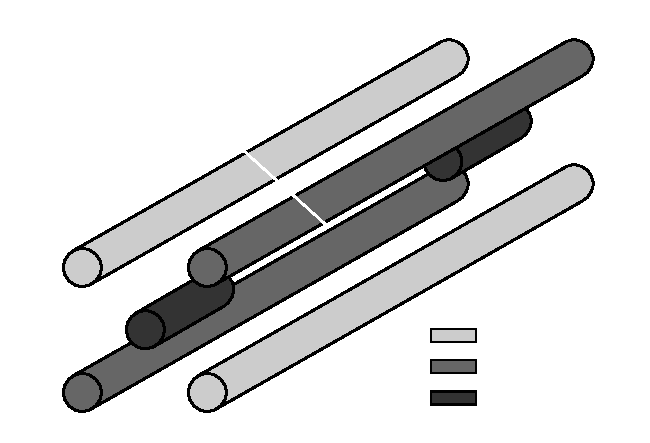
\includegraphics[width=\textwidth]{RF_Trap.pdf}
		\caption{A schematic representation of a simple RF trap. The four electrodes and two endcaps provide the trapping potential.}
		\label{fig:rftrap:schematic}
	\end{subfigure}
	\hfill
	\begin{subfigure}[t]{0.55\textwidth}
		\centering
		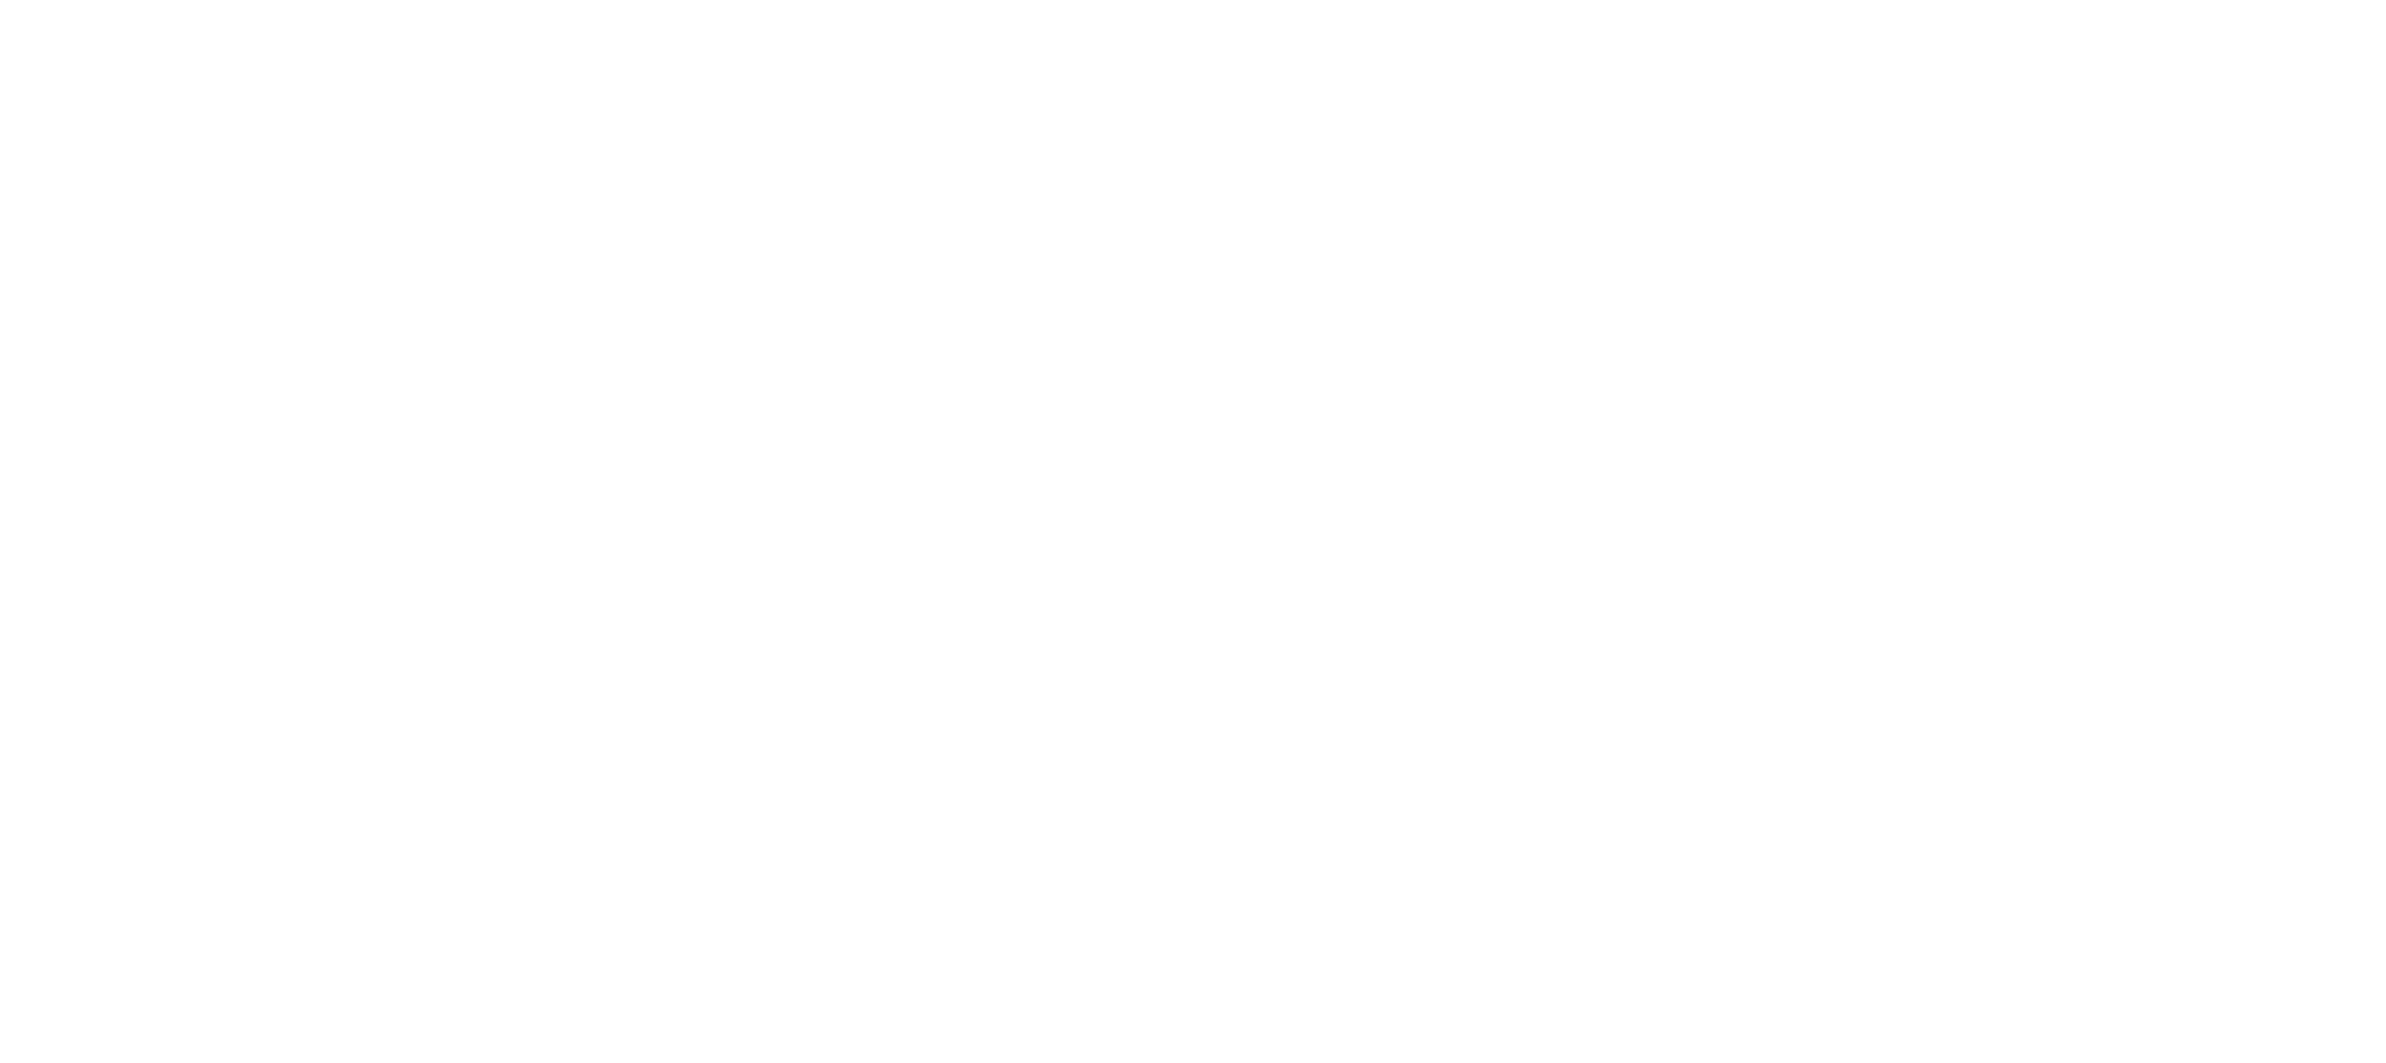
\includegraphics[width=\textwidth]{1ion_Elevels.pdf}
		\caption{Simplified energy structure of an ion in the trap. The qubit states are separated by $\omega_0$ while the motional modes' spacing is dependent on the RF trap's frequency $\nu$.}
		\label{fig:rftrap:estructure}
	\end{subfigure}
	%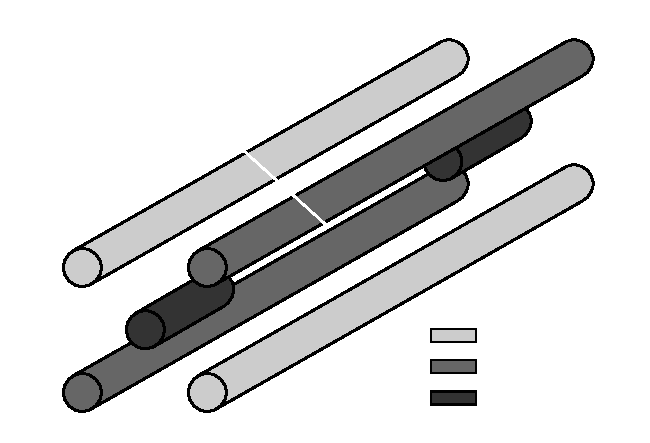
\includegraphics[width=0.7\linewidth]{RF_Trap.pdf}
	\caption[RF Trap schematic and energy]{The static field generated by the endcaps is combined with a fast oscillating field to provide confinement. This usually organises the ions on the trap's axis in a string like pattern \cite{RF_Traps,Charged_Particle_traps_Paul}. This creates an electronic structure pictured in \figref{fig:rftrap:estructure}.}
	\label{fig:rftrap}
\end{figure}
%\end{wrapfigure}

\begin{equation}
	\hat{H}_I = \sum_{j}\frac{\hbar\Omega_j}{2}\hat{\sigma}^{\left(n_j\right)}_+e^{i\eta_j\left(\hat{\tilde{a}} + \hat{\tilde{a}}^\dagger\right)} e^{-i\Delta_jt} + h.c.
	\label{eq:Interaction_H}
\end{equation}

Here we defined $\Delta_j\equiv\omega_j-\omega_0$. We can further examine this Hamiltonian by applying the Lamb-Dicke regime approximation, which is valid for $\langle\eta_j\hat{a}^\dagger\rangle \ll 1$ \cite{MS_gate}. In this limit, we can replace our exponential with the first order expansion, yielding the Hamiltonian:

\begin{equation}
	\hat{H}_I = \sum_{j}\frac{\hbar\Omega_j}{2}\hat{\sigma}^{\left(n_j\right)}_+\left(\mathds{1} + i\eta_j\left(\hat{\tilde{a}} + \hat{\tilde{a}}^\dagger\right)\right)e^{-i\Delta_jt} + h.c.
	\label{eq:Interaction_H_LD}
\end{equation}

This representation highlights two major issues about the system. The most obvious is that coupling to motional sidebands that used to share information between the ions \cite{QIP_Trapped_ions} heavily depends on the vibrational mode of the ions. This dependence will inevitably lead to decoherence of the qubit states, since the necessary timing will then differ for the various thermal occupations. This problem is further intensified by the RF trap's intrinsic property of heating \cite{QIP_Trapped_ions,RF_Traps}, which will lead to collapse of the motional mode if occurs so any entanglement of the qubits with the motional mode must be avoided.

The second issue is not as immediately obvious. This issue arises from the relative coupling strength of the carrier and the sideband transitions. While the central carrier transition will have coupling strength on the order of $\Omega_j$, an illuminating laser will only couple to the  $n$th sideband as an order of $\Omega_j\eta_j^n$. We will see later that this property leads to several unintended consequences.

\section{M\o lmer-S\o rensen Gate}
\label{Background:MS_gate}

\begin{figure}[t!]
	\centering
	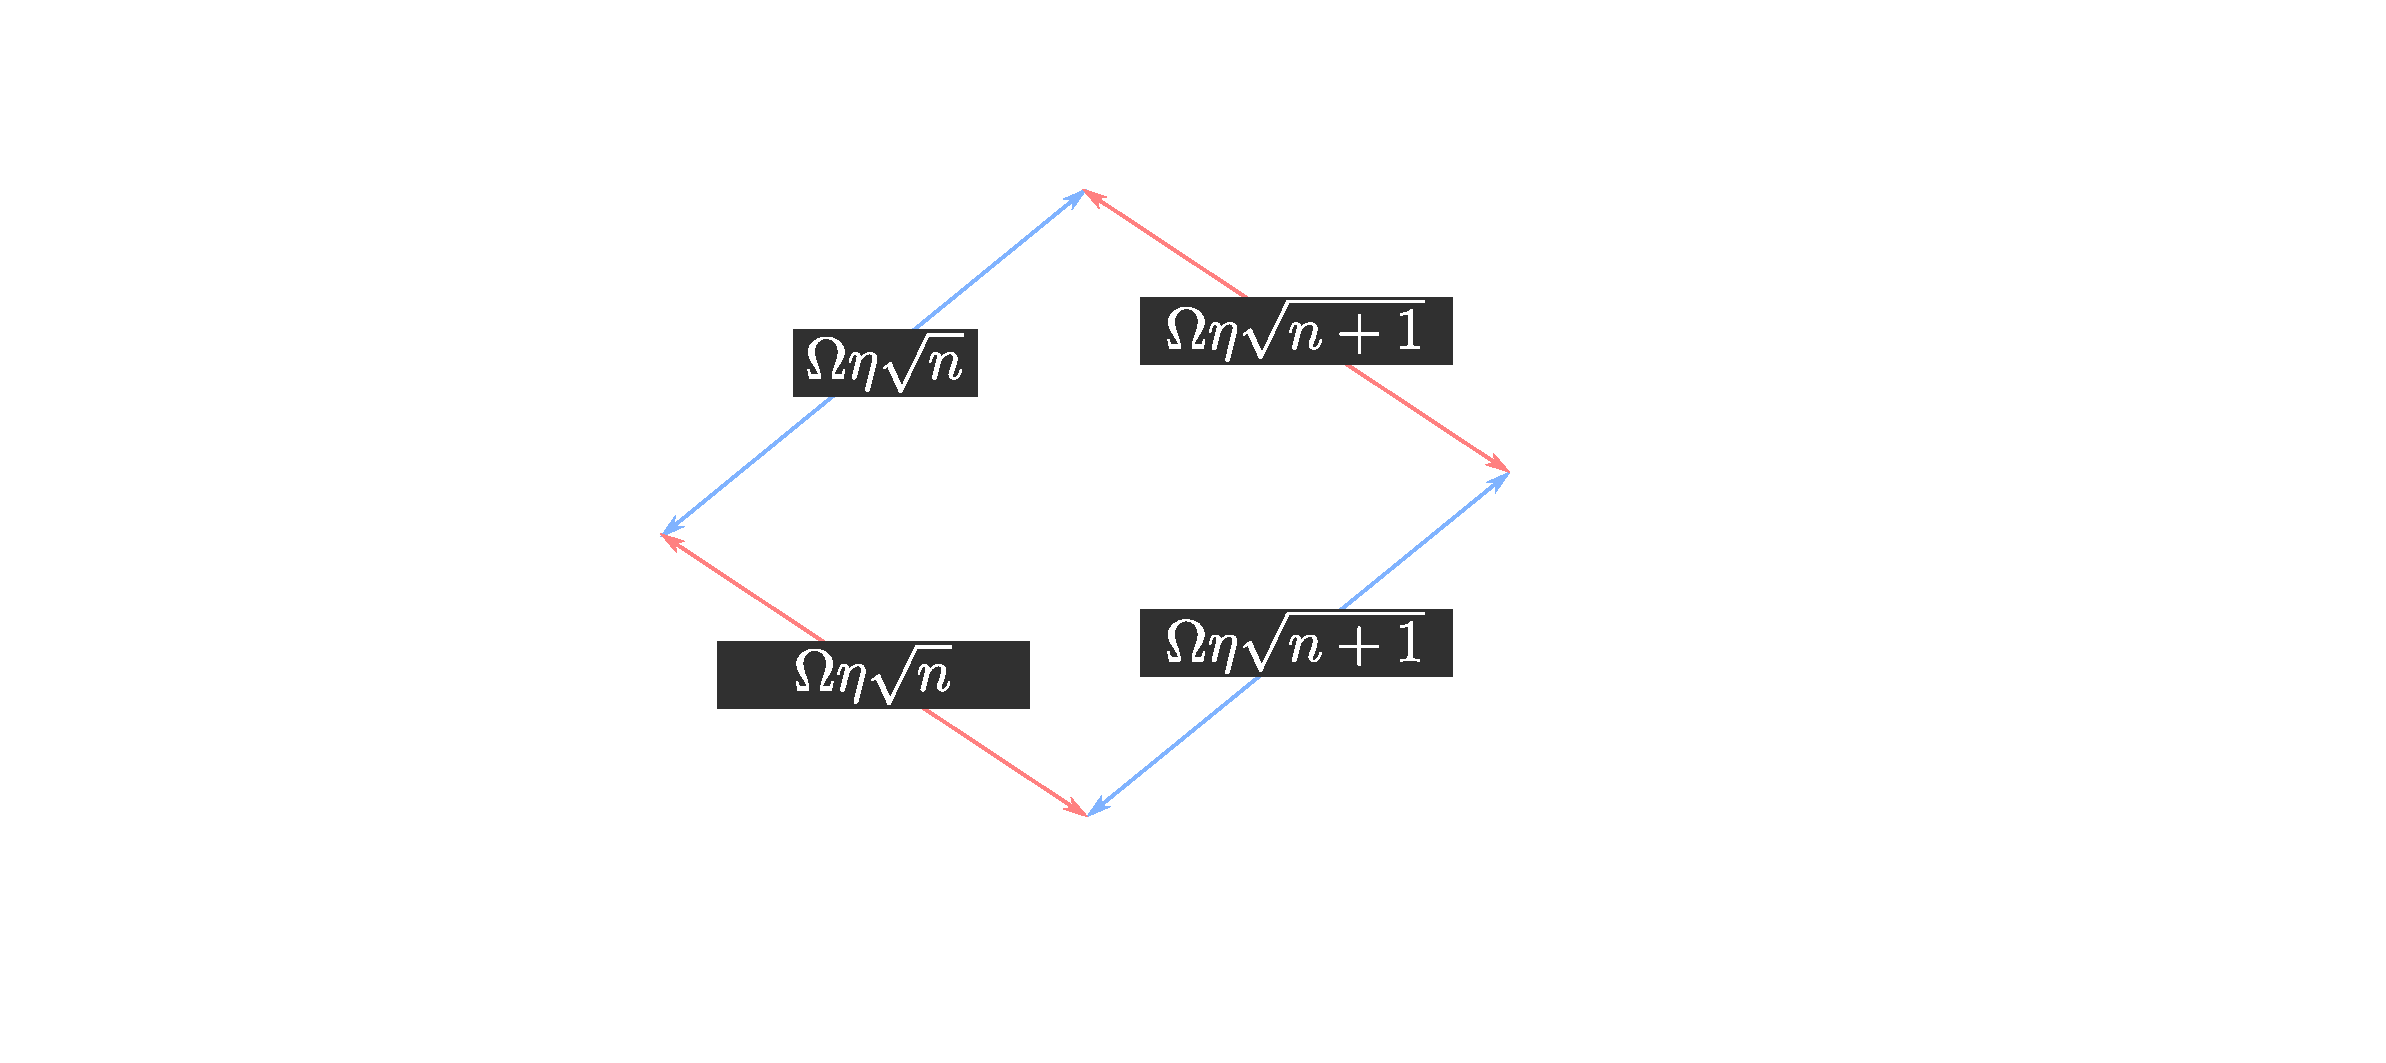
\includegraphics[width=0.9\linewidth]{MS_Gate_Schematic.pdf}
	\caption[MS-gate schematic representation]{A schematic representation of the MS-gate. The lasers drive Raman like transitions between the $|gg,n\rangle$ and $|ee,n\rangle$, through far detuned intermediate states $|eg,n\pm 1\rangle$ and $|ge,n\pm 1\rangle$. The difference in the coupling strength between the two paths available will ensure that the frequency of the transition between the ground and excited states is independent of the motional state $n$.}
	\label{fig:ms_gate_schematic}
\end{figure}

The MS gate solves these problems by addressing the ions in parallel rather than in sequence, as would be standard in a Cirac-Zoller type gate \cite{Cirac_Zoller}. By driving the ions with two laser frequencies, $\Delta_1=\nu-\delta$ and $\Delta_2=-(\nu-\delta)$ simultaneously  This will drive a Raman like \cite{Foot} transition between the $|gg,n\rangle$ and $|ee,n\rangle$ levels by using $|eg,n\pm 1\rangle$ and $|ge,n\pm 1\rangle$ as intermediaries. This is pictured in \figref{fig:ms_gate_schematic}. Alternatively this can also be used to drive transitions between $|eg,n\rangle$ and $|ge,n\rangle$ as discussed within \cite{MS_gate}.

Considering the Lamb-Dicke regime and using second order perturbation theory we can then derive that the transition frequency between the two states will be $\frac{\left(\Omega\eta\right)^2}{2\left(\nu-\delta\right)}$\cite{MS_gate}. As we can see this result is independent of the occupation number $n$ therefore eliminating the gates dependence on it. Furthermore as the system is far detuned from $n\pm1$ no considerable entanglement ever occurs with the thermal state, while we can create an arbitrary entanglement phase between our qubits, creating a gate operation that can be characterised by $|gg\rangle\rightarrow\cos\left(\Phi\right)|gg\rangle + i\sin\left(\Phi\right)|ee\rangle$, where $\Phi$ is a phase parameter dependant on the time we allowed the system to evolve.

The condition that the lasers must be far detuned from the sideband transitions however, is a severe limiting factor in the efficiency of the gate. This requirement slows down gate operation significantly, which exposes the trapped ions to more noise than a faster gate would \cite{Trapped_ion_qbit_toolbox}. To solve these issues, the freedom in choosing $\Phi$, or the entanglement phase can be sacrificed. By allowing the system to briefly transfer population to $|n\pm 1\rangle$ we can speed up entanglement between $|gg\rangle$ and $|ee\rangle$. M\o lmer and S\o rensen have demonstrated that such a setup can be found, decreasing time taken to produce the target $\frac{1}{\sqrt{2}}\left(\left|gg\right\rangle + i\left|ee\right\rangle\right)$ significantly \cite{Fast_MS}. As this gate design is closer to what we are interested in MS gate will refer to this fast design in this thesis.

\section{Physical System}
\label{Background:PhysSys}

As mentioned this work was undertaken to set expectations for a physical implementation of the gates we will discuss in Section \ref{Driving_schemes}. The experiment we are interested in uses $^{40}$Ca$^+$ ions in a linear RF trap as described in \cite{Experiment_setup}. This paper describes the experimental setup that these gates will be implemented on, and as such most our simulations will use the same parameters. For our purposes the most important property of the system is the trap frequency, which is set as $\frac{\nu}{2\pi} \approx 1.1\;\text{MHz}$. A slightly less, but still important parameter is the transition frequency. In this project we modelled our simulations so that the $5S_{1/2,m_j=1/2} \leftrightarrow 4D_{5/2,m_j=1/2}$ transition would be our qubit state, which is a long lived qubit due to the decay being forbidden under the electric dipole selection rules \cite{Foot}. This transition has $\frac{\omega_0}{2\pi} \approx 411\;\text{THz}$, which can then be used to calculate the Lamb-Dicke parameter for the setup, which were consistent the figure presented in \cite{Experiment_setup}. At this point for convenience a slight approximation can be made. Since all lasers would be parallel to the trap's axis, and had similar wavenumbers we have decided that ${\eta_j \approx \eta}$, where $\eta$ was defined as the Lamb-Dicke parameter of a laser resonant to the carrier transition. While a scheme where this assumption does not hold might be interesting to pursue, that is beyond the scope of this work.

%%%%%%%%%%%%%%%%%%%%%%
\chapter{Simulation Framework}
\label{Sim_Framework}

To evaluate the gate designs we had to simulate realistic conditions, which we would expect to see in an experimental setting. To achieve this we decided to use Qutip \cite{QuTip1,QuTip2}, a simulational framework used to model problems relating to quantum systems. We used their numerical solvers to integrate the von Neumann equation \cite{Shankar_QM} ${\der{\hat{\rho}}{t} = -\frac{i}{\hbar}\left[\hat{H},\hat{\rho}\right]}$, where we used the Hamiltonian from \eref{eq:RF_Trap_H_driven} and $\rho$ marks the density matrix.

\begin{figure}[b!]
	\centering
	\begin{subfigure}[t]{0.475\textwidth}
		\centering
		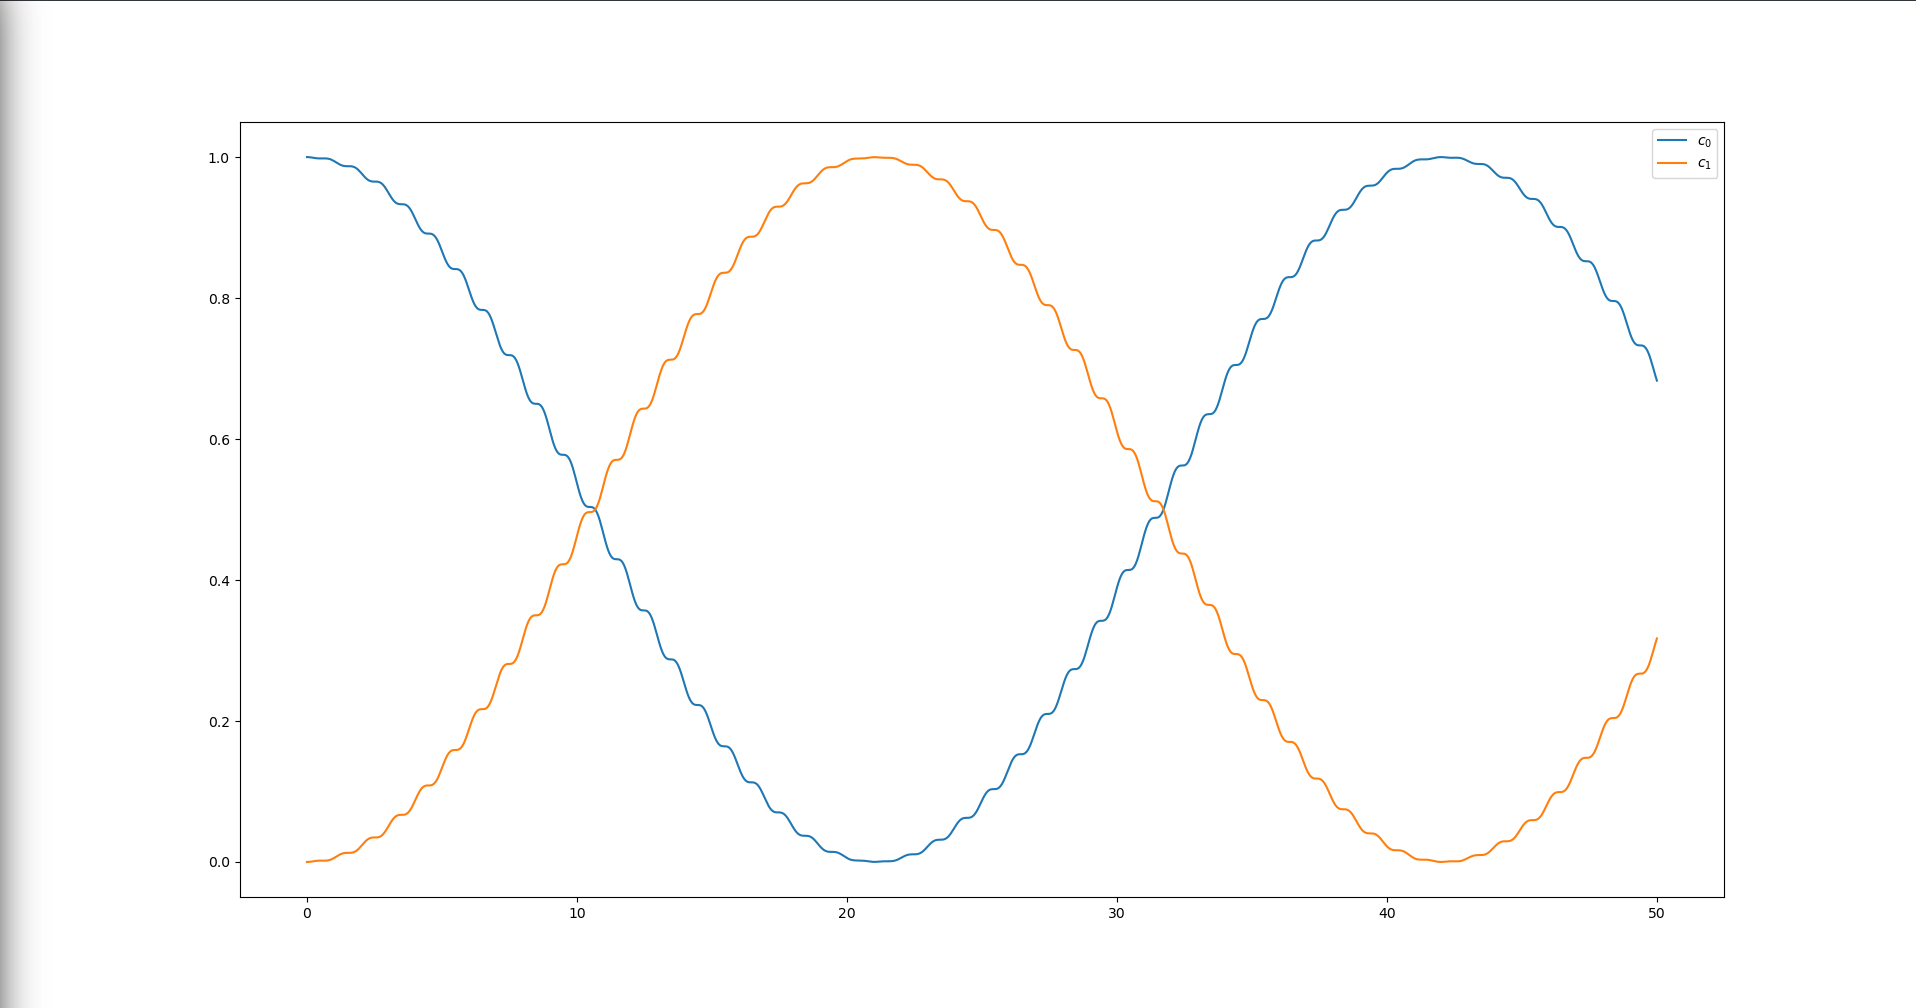
\includegraphics[width=\textwidth]{Rabi.pdf}
		\caption{Simulated two level system population in presence of a resonant driving field with Rabi frequency of $\frac{\Omega}{2\pi} = 1000\;\text{Hz}$. The two levels' population is shown as the diagonal elements in the density matrix $\hat{\rho}$.}
		\label{fig:rabi:measured}
	\end{subfigure}
	\hfill
	\begin{subfigure}[t]{0.475\textwidth}
		\centering
		\includegraphics[width=\textwidth]{Rabi_residual.pdf}
		\caption{Error in the simulation as characterised by the inaccuracy of $\langle e|\hat{\rho}|g\rangle$ compared to its theoretical value. As we can see our simulation differs in a mostly negligible fashion that is expected of any numerical solution.}
		\label{fig:rabi:residual}
	\end{subfigure}
	%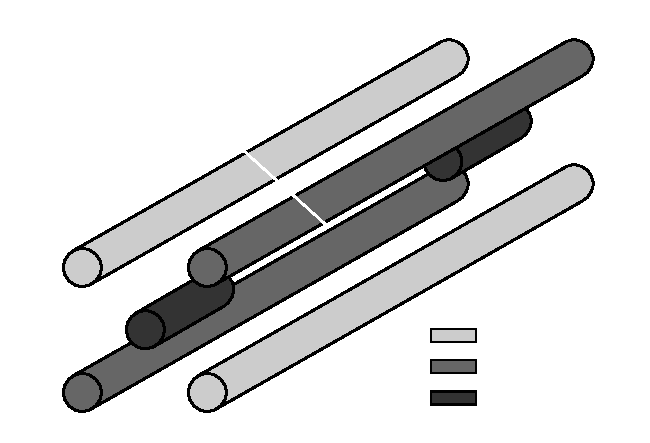
\includegraphics[width=0.7\linewidth]{RF_Trap.pdf}
	\caption[Rabi oscillation simulation]{Benchmark simulation involving Rabi oscillations. For these parameters $\langle e|\hat{\rho}|e\rangle = \sin^2\left(\frac{2\pi1000}{2}t\right)$ is expected, which is what can be observed.}
	\label{fig:rabi}
\end{figure}

To confirm that our simulation had no artefacts we used two benchmarks. The first was a confirmation of the solver producing high precision data, for which a simple simulation of a Rabi oscillation was used. For this to not be tainted by motional modes we have set $\eta =0$. The second test was designed to find bugs in the expansion of $e^{i\eta\left(\hat{\tilde{a}}+\hat{\tilde{a}}^\dagger\right)}$. Testing for the second artefact is harder since the Hamiltonian where this term is fully expanded is difficult to solve analytically. To circumvent this we decided to reproduce Figure 2 from \cite{MS_gate}. This allowed us to compare our simulations performance to established work. The results of these simulations van be seen in Figures \ref{fig:rabi} and \ref{fig:msbench}.

We can see that both our simulations agree with either the theoretical prediction. In the case of the Rabi oscillation we are able to see the inaccuracies the numerical integrator introduces to our result. For the MS gate's case we can not make such a precise comparison. This is due to the fact that the data is not only not available, but it would also not be exact for our simulation, as they have used the Lamb-Dicke regime approximation. While this would change the results slightly, we do not believe it affects them severely enough that our results will accidentally align with theirs, which would invalidate this benchmark.

An other thing to consider was the performance of our simulation. Unfortunately even though the full Hamiltonian would be preferred, sometimes simulating a system that complex would be too computationally intensive. To illustrate this we can express motional coupling of the Hamiltonian can be expanded into a form:

\begin{equation}
	e^{i\eta\left(\hat{\tilde{a}}+\hat{\tilde{a}}^\dagger\right)} = \sum_{k=-\infty}^\infty \hat{c}_k e^{-ik\nu t}
	\label{eq:Mot_exp}
\end{equation}

\begin{figure}[t!]
	\centering
	\begin{subfigure}[t]{0.475\textwidth}
		\centering
		\includegraphics[width=\textwidth]{MS_Gate_Benchmark.pdf}
		\caption{Simulation of the standard MS gate. The density matrix elements we are most interested in are plotted. The real part is displayed as a solid while the imaginary component is plotted as a dotted line.}
		\label{fig:msbench:measured}
	\end{subfigure}
	\hfill
	\begin{subfigure}[t]{0.475\textwidth}
		\centering
		\includegraphics[width=\textwidth]{MS_Gate_paper.pdf}
		\caption{The original simulation presented reproduced from \cite{MS_gate}. The solid line represents $Re\left(\langle gg|\hat{\rho}| gg\right)$, the long dashed line is $Re\left(\langle ee|\hat{\rho}|ee\rangle\right)$ and the short dashed line is $Im\left(\langle gg|\hat{\rho}|ee\rangle\right)$.}
		\label{fig:msbench:original}
	\end{subfigure}
	%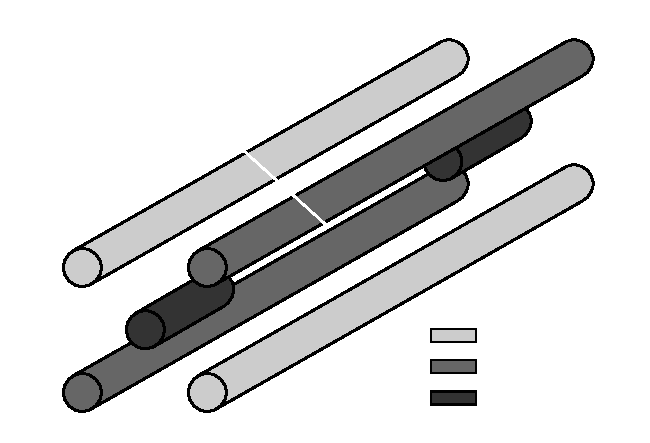
\includegraphics[width=0.7\linewidth]{RF_Trap.pdf}
	\caption[MS Gate benchmark]{Benchmark simulation reproducing Figure 2 from \cite{MS_gate}. As we can see the timing and shape of both curves are in agreement, furthermore both exhibit the same high frequency oscillations toward the peak of $\langle gg|\hat{\rho}|gg\rangle$.}
	\label{fig:msbench}
\end{figure}

Here each term represents a transition on the motional modes, with $\hat{c}_k$ facilitating a transition between $|n\rangle$ and $|n+k\rangle$. While this relationship does not hold perfectly it can be beneficial to consider $\langle\hat{c}_k\rangle\approx\langle\eta^k\hat{a}^{\dagger k}\rangle$. This approximation can be seen, by expanding the exponential manually and for each diagonal only considering the first term. While this is only a heuristic to provide us insight into computational difficulties, it is a very useful tool, when considering the relative coupling strengths, since these first terms would be dominant if $\langle\eta^k\hat{a}^{\dagger k}\rangle\ll 1$. From this it is very easy to see how small the coupling of the laser is to far off sidebands\cite{Charged_Particle_traps_Cooling}. This weak coupling issue is compounded by the fact that these far detuned transitions with large $|\Delta_j -k\nu|$ also induce fast small amplitude oscillations. These do not influence the end result in any way, but slow down computation significantly. One way of dealing with this is to ignore transitions, that are "off resonant", i.e. when the laser is far detuned from them, which is the tactic used by many papers on the subject\cite{Cardioid,MS_gate,Fast_MS,SC_Paper}. As we will see later this is not exactly an optimal solution since it loses valuable information about the feasibility of these gates. Instead we introduced a culling condition into our Hamiltonian:

\begin{equation}
	|k\nu-\Delta_j| > 50|\Omega_j|\cdot 2^{|k|}\eta^{|k-1|}
	\label{eq:culling}
\end{equation}

Any term in \eref{eq:Mot_exp} that cannot fullfill this condition will be discarded. This condition is generous enough that for our purposes, the results are indistinguishable from a full Hamiltonian simulation. We have decided to use a cutoff of $|\Delta_j -k\nu| = 50\Omega_j$ as detuning since we observed in preliminary  tests that this produced reliable results. We also included factors of $2\eta$ to bias against far sidebands, which is a condition resulting from the naive expansion of $\hat{c}_k$ in \eref{eq:Mot_exp} for $n=4$. While we found that these parameters, and formula produced accurate results, we concede that the choice of cutoff values are somewhat arbitrary and we advise anyone to carefully evaluate this approach if used.

Finally to characterise the designs we will be using the infidelity of the final state. This can be expressed as $1-\langle\Psi|\hat{\rho}|\Psi\rangle$, where $\Psi$ is the target state. This will generally be $\Psi = \frac{1}{\sqrt{2}}\left(\left|gg\right\rangle + i\left|ee\right\rangle\right)$, but as we will see later some gates allow flexibility beyond this.

The code used to run the simulations along with some of the configurations used to generate plots is made public in a repository \cite{Github} and after submission will only see minor changes like commenting and removing legacy sections. The unaltered version will be kept on the "Thesis" branch. This repository contains original code produced by the author for the purpose of simulating the fidelity of the driving schemes presented below. The simulations were produced by the three files \texttt{Seq\_core.py}, \texttt{Var\_core.py} and \texttt{Time\_core.py}. The first simulates pulse sequences and stores the evolution of the states, while the last two provide wrappers to vary some parameter about the simulation and stores only the end result.

%%%%%%%%%%%%%%%%%%%%%%%%%%%%%%%%%%%%
\chapter{Explored Driving Schemes}
\label{Driving_schemes}

\section{Strong Coupling Gate}
\label{Driving_schemes:SC}

It is clear that the motional sidebands, characterised by the exponential ${e^{i\eta\left(\hat{\tilde{a}}+\hat{\tilde{a}}^\dagger\right)}}$ play a key role in the driving scheme's fidelity. One major issue with the MS gate however is that this exponential is only very naively expanded into the Lamb-Dicke approximation\cite{Fast_MS}. While this allows for a simpler theoretical treatment of the system it fundamentally introduces errors stemming from the inaccuracies of such a treatment. An obvious solution is to include additional terms in the exponential's treatment. This is the approach taken by \cite{SC_Paper}, where an exact expansion is used in place of the simpler Lamb-Dicke approximation. Using the notation provided in \eref{eq:Mot_exp} we can represent this expansion as \cite{SC_Paper}:

\begin{equation}
	\hat{c}_k = e^{-\frac{\eta^2}{2}}\sum_{n=0}^\infty \left(i\eta\right)^{2n+k}\frac{\hat{a}^{\dagger n+k}}{\left(n+k\right)!}\frac{\hat{a}^{n}}{n!}
	\label{eq:SC_expansion}
\end{equation}

Here $k > 0$ and $\hat{c}_{-k} = \hat{c}_k^\dagger$. While this expansion is exact, there is no easy way to deal with a Hamiltonian including this. In the paper this issue is solved by iteratively computing a propagator, which is the product of several time dependent sub-propagators: $\hat{U} \approx \hat{V}_d = \prod_{n=0}^{d}\hat{U}_d$. From a propagator of this form we can generate a new Hamiltonian ${\hat{H}_{j+1} = \hat{V}_d^\dagger \hat{H}_I^{'} \hat{V}_d - i\hat{V}_d^\dagger\hat{\dot{V}}_d}$, which only includes terms until $\eta^{j+1}$. Here $\hat{H}_I^{'}$ is the Hamiltonian from Equation \eqref{eq:Interaction_H} without the off resonant transitions. These were ignored as including them would complicate derivation too much. We can then produce a new propagator term $\hat{U}_d = e^{-i\int_{0}^{t}\hat{H}_d\text{d}t'}$. Using the Lamb-Dicke approximation as $\hat{H}_0$ we can construct a propagator to arbitrary degrees of $\eta$\cite{SC_Paper}.

From this we can then require that, at gate time, $\hat{V}_d=e^{i\Phi\hat{S}_y^2}$, which is referred to as the entangling condition. This will ensure that our final state ${\cos\left(\Phi\right)|gg\rangle + i\sin\left(\Phi\right)|ee\rangle}$ does not have unwanted contributions from higher order terms dependant on $n$. To eliminate other terms at gate time, they utilise higher order transitions, meaning that in addition to the first sideband driving of the MS gate, they add extra terms for farther off sidebands. As an example eliminating terms with order $\eta^4$ requires driving second order, while $\eta^6$ needs third order sidebands. The expressions that need to vanish also quickly increase as the approximation is expanded to higher order, and since these expressions are too long to be included here, we won't be including them, but they are mentioned in \cite{SC_Paper} with the exact formulation in \cite{SC_github}. This will lift the Lamb-Dicke regime requirement, $\langle\eta\hat{a}^{\dagger}\rangle\ll 1$, allowing high fidelity computation with hotter states.

In the original paper discussing the design, they provide two proof of concept driving profiles. One utilising two and an other using three sidebands. Unfortunately when we consider terms that are off resonant their fidelity is quickly lost, but if gates with speed on the order of $100\;\mu\text{s}$ are needed, these terms become necessary to consider. Due to this we will only be including the two sideband case as a baseline for results in Section \ref{Driving_schemes:Compound} and for the ideal operation of a three sideband case one can refer to \cite{SC_Paper}.

The two sideband proof of concept provided in \cite{SC_Paper} can be brought into our formulation as 4 lasers driving each of our ions. Using the definition we established in Sections \ref{Background:RF_Trap} and \ref{Sim_Framework} the parameters will be $\Delta_0 = -\Delta_1 = \nu - 2\delta$ and $\Delta_2 = -\Delta_3 = 2\nu-\delta$. These lasers will have coupling strengths ${\Omega_1 = \Omega_2 = -\Omega_3 = \Omega_4 = ie^{\frac{\eta^2}{2}}\Omega}$, where $\Omega$ and $\delta$ are parameters related by the entangling condition ${3\eta^6(\frac{\Omega}{\delta})^4 - (1 + \eta^2)\eta^2(\frac{\Omega}{\delta})^2 + \frac{\Phi}{\pi} = 0}$. This will produce the expected state in $t_g = \frac{2\pi}{\delta}$.

We have then compared this strong coupling gate design with the MS gate, for which the results are seen in Figure \ref{fig:sc2:comparison}. In this simulation, to highlight the benefits of the strong coupling gate, by only considering the on resonant terms. We however also show in Figure \ref{fig:sc2:time} that including these terms are detrimental to the gate's operation. If the gate is only weakly driven, these issues can be avoided, but that comes at the cost of gate speed.

Unfortunately this design does not seem to be reasonably implementable due to these concerns about off resonant transitions.

\begin{figure}[t!]
	\centering
	\begin{subfigure}[t]{0.475\textwidth}
		\centering
		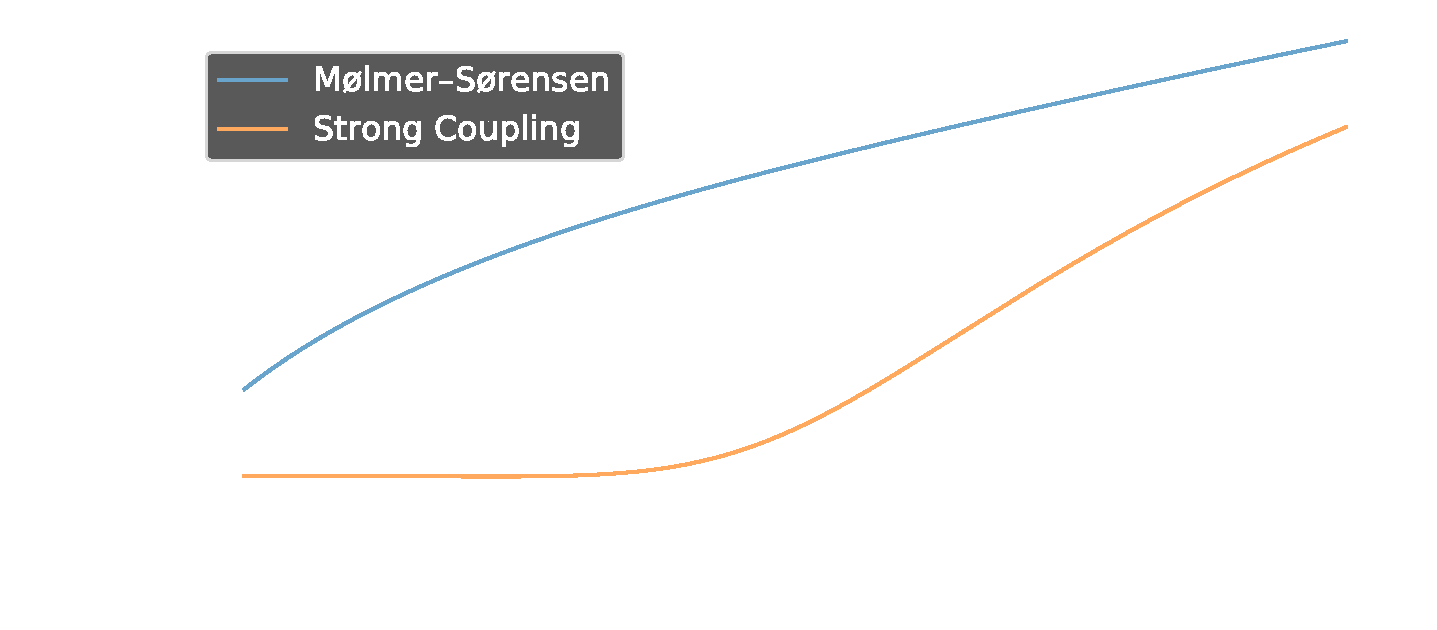
\includegraphics[width=\textwidth]{SC2_therm.pdf}
		\caption{Comparison between the MS gate's and the strong coupling scheme's effectiveness against higher temperature ions, if only on resonant terms are included in the Hamiltonian. It is easily seen that the strong coupling design is more robust against these errors.}
		\label{fig:sc2:comparison}
	\end{subfigure}
	\hfill
	\begin{subfigure}[t]{0.475\textwidth}
		\centering
		\includegraphics[width=\textwidth]{SC2_off_res.pdf}
		\caption{A time scan of the strong coupling gate's operation. The initial state was set as $|gg,0\rangle$. The strong driving induces fast oscillations on the carrier, yielding fast off resonant transitions. These reduce the final fidelity to $~98\%$ with the fast oscillations providing the potential to lose up to $3\%$ more.}
		\label{fig:sc2:time}
	\end{subfigure}
	%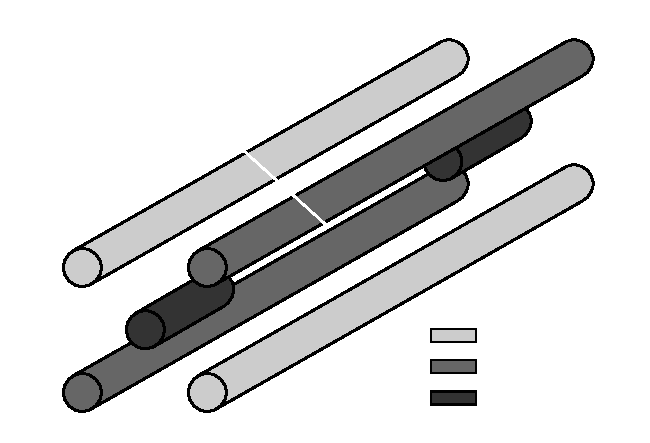
\includegraphics[width=0.7\linewidth]{RF_Trap.pdf}
	\caption[Strong coupling design]{Comparison between the effectiveness of the strong coupling gate, while only simulating on resonant (left). On the right we provide an example why this on resonant term approximation is flawed. The parameters were $\Omega_0 = 0.1\nu$ and $\Phi=0.5\pi$ for both cases, but this is more relevant to the right plot, since the left one ignores off resonant terms.}
	\label{fig:sc2}
\end{figure}

\section{Cardioid Gate}
\label{Driving_schemes:Cardioid}

An other design aiming to improve upon the MS gate is the cardioid family of gates. They are part of a larger ensemble of similarly designed gates, with similar properties. The idea behind their construction is that multiple tones of lasers are driven on the same sideband, which introduces further degrees of freedom that can be manipulated to produce gates that are robust against some external effects \cite{Cardioid}. In their original formulation they provide an example of resistance against timing errors.

The gates they propose have the general form $\Delta_{2i} = -\Delta_{2i + 1} = \nu - n_i\delta$, where $\delta$ is a parameter related to gate time by the familiar expression $t_g = \frac{2\pi}{\delta}$. Their relative intensities can then be expressed as $\Omega_{2i} = \Omega_{2i + 1} = r_i\Omega$, where  $\Omega = \frac{\delta}{2\eta}$ and $\sum_{i}\frac{r_i^2}{n_i} = 1$. They found these conditions after integrating the Lamb-Dicke regime Hamiltonian, while neglecting the off resonant carrier terms \cite{Cardioid}. This raises problems similar to the ones we have seen in the strong coupling gate's case. One promising proposition is that the extra degrees of freedom we control can be used to reduce these errors.

The cardioid is one such gate design. It is characterised by 2 tones on both the red and blue sidebands, with $r_0 = -r_1$ as well as a free choice of $n_0$ and $n_1$. We can then introduce these terms into Equation \eqref{eq:Interaction_H_LD}:

\begin{equation}
	\hat{H}_I = \sum_j \frac{\hbar r_j\Omega}{2}(\hat{S}_x (e^{i(\nu - n_j\delta)t} + h.c.) + \eta \hat{S}_y (\hat{a}e^{in_j\delta t} + h.c))
	\label{eq:Cardioid}
\end{equation}

Where we have ignored the far resonant sideband terms, such as the red sideband driving the blue sideband off resonantly. While we could represent the propagator as $\hat{U}\approx \prod_0^t e^{-i\int_{t}^{t + \Delta t}\hat{H}_I\text{d}t'}$, the treatment and evaluation of this expression would be extremely laborious and this work's scope is too limited for such a discussion. Alternatively we can take an other, more naive approach. Instead of using the extra degrees of freedom to reduce the overall loss of fidelity that happens during gate operation, we can focus on the noise generated at gate time. This noise is extremely problematic, due to it adding a randomness to the final state, with the only remedy being very precise timing. By requiring the first term to disappear at gate time, we can ensure that these unwanted transitions disappear as well.It is easy to see that for a cardioid gate, the first term will become proportional to $\cos(\frac{(n_0 - n_1)\delta}{2}t)$. Since $n_0, n_1 \in \mathbb{Z}$, this will ensure that at $t_g = \frac{2\pi}{\delta}$ this expression becomes zero. This is while still providing resistance against timing errors as was discussed in \cite{Cardioid}.

We decided that out of the variety of cardioid gates the Cardioid($4$, $6$), would be explored. Here numbers represent the values of $n_i$. As a note, since all gates in this family exhibit the behaviour of reducing off resonant carrier transitions near gate time, our choice of focusing our simulation on Cardioid($4$, $6$) was somewhat arbitrary. This is due to us wanting to provide an example of these beneficial properties as well as its shortcomings. Figure \ref{fig:cardioid} highlights how the cardioid scheme improves the fidelity near gate time, but does nothing to combat thermal effects.

\begin{figure}[t!]
	\centering
	\begin{subfigure}[t]{0.475\textwidth}
		\centering
		\includegraphics[width=\textwidth]{Card_time.pdf}
		\caption{Simulation the full expansion of the Hamiltonian. As we can see both gates present with oscillations far from gate time, but in the case of the cardioid, this oscillation disappears stabilising the curve around $0.1\%$ infidelity. The MS gate however remains oscillating introducing a possible loss in fidelity of $\sim 2\%$ if the gate time is implemented slightly incorrectly. Both systems started in $|gg,0\rangle$.}
		\label{fig:cardioid:full}
	\end{subfigure}
	\hfill
	\begin{subfigure}[t]{0.475\textwidth}
		\centering
		\includegraphics[width=\textwidth]{Card_therm.pdf}
		\caption{Fidelity comparison between the Cardioid($4$, $6$) and MS gates under different ion temperatures. For the results to be without noise, we have ignored off resonant terms. As we can see the cardioid still suffers from the same loss of fidelity that is prevalent in the MS gate's case.}
		\label{fig:cardioid:therm}
	\end{subfigure}
	%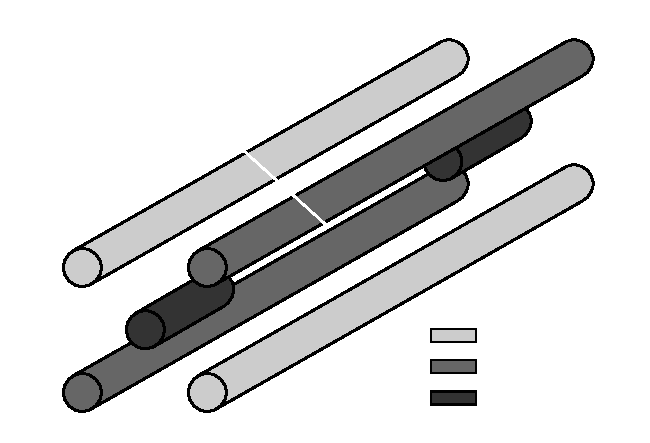
\includegraphics[width=0.7\linewidth]{RF_Trap.pdf}
	\caption[Cardioid gate comparison]{Comparison between the fidelity the MS gate and the Cardioid($4$, $6$). The left plot highlights the improvement the cardioid scheme has in a strongly driven ($\Omega = 0.1\nu$) case. The right plot however shows that since it does not expand the Hamiltonian to high orders, it is not resistant against thermal effects.}
	\label{fig:cardioid}
\end{figure}

\section{Compound Gate}
\label{Driving_schemes:Compound}

Finally we have aimed to create a gate design that has the benefits of both the strong coupling and the cardioid scheme. We have used the expansion detailed in Section \ref{Driving_schemes:SC}. We have done this by creating a wrapper around the conditions provided in \cite{SC_github}, and feeding it parametrised versions of driving terms. This was done using Mathematica, for which the code is included in \texttt{SC2.nb}. Here the terms on the first sideband were set to mimic a chosen driving scheme, while the second sideband was used to reduce the necessary terms in our equation to zero. The solution we used however is far from automatic and there does not seem to be a simple way of making it automatic. This also did not produce compound schemes for all gates we tried. As an example, we have originally experimented with a Cardioid($2$, $3$) gate, however we could not find a second sideband driving, which would reduce the unwanted propagator terms to zero.

Due to the manual nature of this parameter variation, we also decided that three sideband driving cases would not be attempted. This decision is mainly due to the fact that a three sideband driving would require a staggering number of terms to become zero, compared to the $12$, which is needed for a two sideband design. We also believed that a three sideband gate would not improve the final gate's fidelity drastically as the extra driving terms would possibly create more noise from off resonant transitions. This is however only speculative on trends noticeable in Figure \ref{fig:comparison}. In it we can see that even though the strong coupling should outperform the MS gate, it only starts approaching a similar level of fidelity as the driving term becomes weaker, which reduces the prevalence of off resonant transitions we do not mitigate against. An example of this would be a second sideband laser driving a first sideband transition off resonantly.

The gate we have found a working extension using the strong coupling constraints was the Cardioid($4$, $6$). Using the same $4$ lasers on the first order as discussed in Section \ref{Driving_schemes:Cardioid} and adding a $4$ extra driving terms on the second sideband would reduce the unwanted terms in the propagator to zero. The driving scheme's breakdown can be found in Table \ref{tab:Compound}.


\begin{table}[t!]
	\centering
	\begin{tabular}{c||cccc|cc}
		\hline
		$\Delta_i$ & $\pm(\nu - 4\delta)$ & $\pm(\nu - 4\delta)$ & $\pm(\nu - 6\delta)$ & $-(\nu - 6\delta)$ & $2\nu - \delta$ & $-(2\nu - \delta)$ & $2\nu - 3\delta$ & $-(2\nu - 3\delta)$ \\
		\hline
		$\Omega_i$ & $\Omega'$ & $-\Omega'$ & $\Omega'$ & $-\Omega'$& $\sqrt{\frac{5}{8}}\Omega'$ & $-\sqrt{\frac{5}{8}}\Omega'$\\
		\hline
	\end{tabular}
	\caption{The relative driving strengths and detunings required for the compound gate's operation. We have defined $\Omega' = ie^{\frac{\eta^2}{2}}$ for a more compact description.}
	\label{tab:Compound}
\end{table}

\begin{figure}[b!]
	\centering
	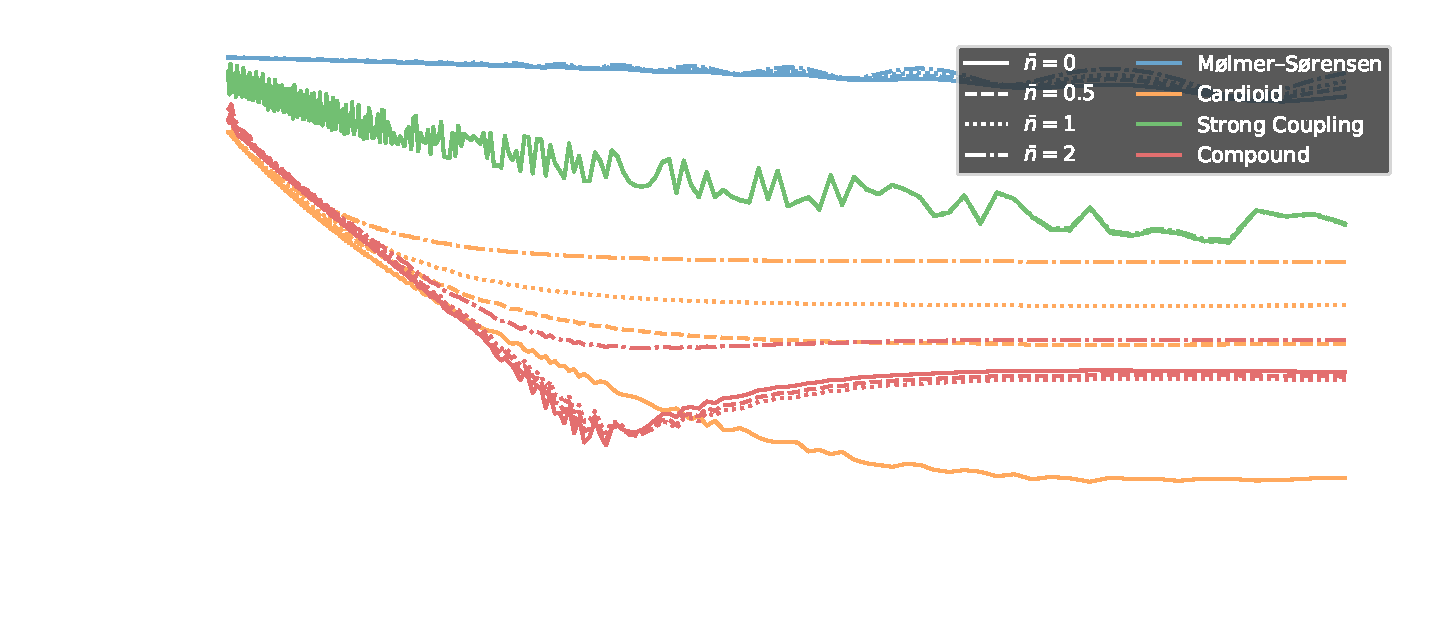
\includegraphics[width=0.9\linewidth]{Comparison.pdf}
	\caption[Gate comparison]{Comparison between the various driving schemes. The colour indicates the type of gate, while its drawing style shows the initial thermal occupation simulated. As we can see both the MS and the strong coupling gates suffer from large fluctuations in fidelity, most likely due to off resonant carrier transitions. The compound and cardioid schemes have minor noise visible as well, and these are most likely due to off resonant transitions on some sideband. Since the driving terms couple to the sidebands less strongly, their perturbation is much weaker.}
	\label{fig:comparison}
\end{figure}

\section{Dynamical Decoupling}
\label{Driving_schemes:DD}

Finally I would like to talk about an addition to the previous schemes. The dynamical decoupling (DD) scheme is aimed to eliminate infidelity from errors in the qubits' transition frequencies. These errors arise naturally from electric and magnetic interferences inducing Zeeman and Stark shifts []. Including these errods the original interaction Hamiltonian from eref can be modified as:

Where $\xi_i$ is the error in the $i$th qubit's frequency.  We can include a strong carrier driving of form $ $, and then moving into the interaction picture with respect to this new term, we find that:

The most important result is that if $[\hat{H}_I,\hat{S}_y]=0$, then our gate operation is unaffected by the addition of this new term. As it turns out this is the case for both our compund and the strong coupling gates. For the M\o lmer-S\o rensen and cardioid gates a similar driving term can be used to produce similar results, detailed in the original paper []. We can also see that for $t_g, \xi_i \ll \Omega_c$ the error ter reduces to fast oscillations. This Hamiltoinan however will not coincide with the lab frame hamiltonian, only when $\Omega_c t_g = 2\pi n$ for $n \in \mathbb{Z}$.

As discussed in [] this requirement can be avoided, by implementing the gate in two equal time phases and applying a $\pi$ pulse between them. This is easily doable in the case of the strong coupling gates including our compund gate.
We aimed to eliminate noise on the order of $1000\;\text{Hz}$ or $\sim 6300\;\text{s}^{-1}$.

%%%%%%%%%%%%%%%%%%%%%%%%%%%%%%%%%%%%
\chapter{Conclusion}
\label{Conclusion}

%% bibliography
\bibliographystyle{ieeetran}
\bibliography{sources}

\end{document}